\documentclass[tikz, border=12pt]{standalone}
\usepackage[utf8]{inputenc}
\usepackage[T5]{fontenc}
\usepackage{lmodern}
\usepackage{xcolor}
\usepackage{graphicx}
\usetikzlibrary{positioning, calc, arrows}

% Bảng màu thanh nhã chuẩn quốc tế
\definecolor{boxBorder}{RGB}{180, 195, 215}
\definecolor{boxBg}{RGB}{250, 252, 255}
\definecolor{titleNavy}{RGB}{20, 50, 110}
\definecolor{arrowColor}{RGB}{50, 65, 85}

\begin{document}
\begin{tikzpicture}[
  >=stealth,
  font=\sffamily,
  stageCard/.style={
    draw=boxBorder,
    line width=0.9pt,
    fill=boxBg,
    rounded corners=6pt,
    align=center,
    inner sep=5pt
  },
  arrowMain/.style={
    ->,
    line width=1.3pt,
    draw=arrowColor
  },
  arrowDash/.style={
    ->,
    dashed,
    line width=1.2pt,
    draw=arrowColor
  },
  tagLbl/.style={
    font=\small\bfseries,
    fill=white,
    inner sep=3.0pt,
    rounded corners=3pt,
    draw=gray!35,
    line width=0.5pt,
    text=arrowColor
  }
]

% 1. HÀNG KHỐI CHÍNH (3 Khối ngang cân đối hoàn hảo)
% Khối 1: Bàn tay mang nẹp
\node[stageCard, text width=4.5cm, minimum height=4.2cm] (hand) at (-5.6, 0) {
  {\bfseries\normalsize\color{titleNavy} BÀN TAY MANG NẸP}\\[4pt]
  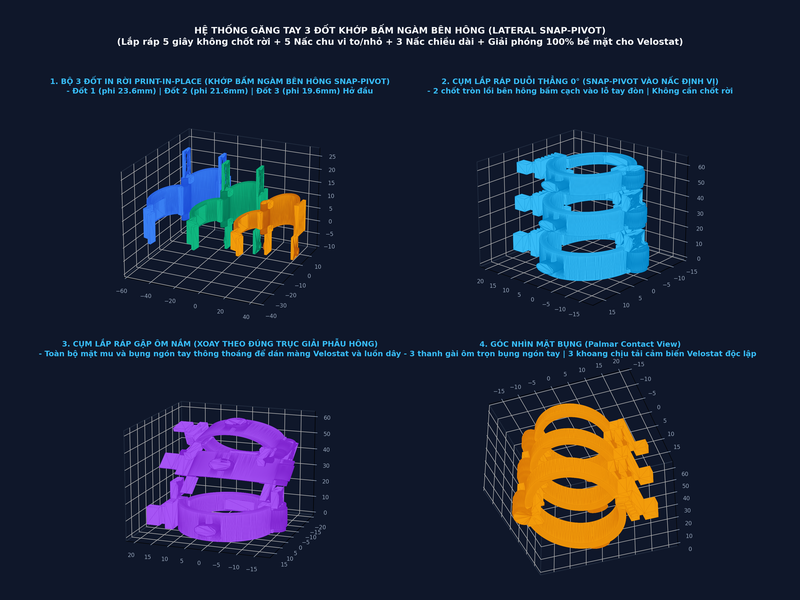
\includegraphics[width=4.1cm, height=2.6cm, keepaspectratio]{assets/splint_3d.png}\\[4pt]
  {\footnotesize 16 Ô Velostat vi sai + 3 Flex}
};

% Khối 2: Bộ điều khiển trung tâm
\node[stageCard, text width=4.5cm, minimum height=4.2cm] (ctrl) at (0, 0) {
  {\bfseries\normalsize\color{titleNavy} BỘ ĐIỀU KHIỂN}\\[4pt]
  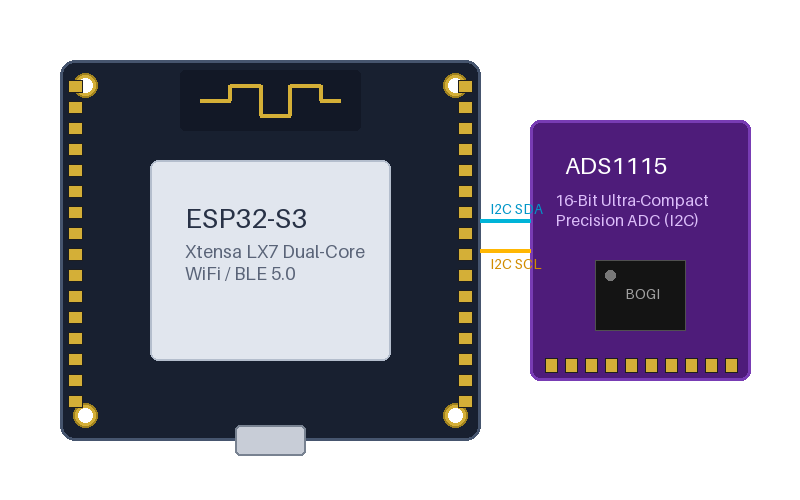
\includegraphics[width=4.1cm, height=2.6cm, keepaspectratio]{assets/controller_ads_board.png}\\[4pt]
  {\footnotesize ESP32-S3 + ADS1115 (DSP \& AAN)}
};

% Khối 3: Trợ lực cơ học servo
\node[stageCard, text width=4.5cm, minimum height=4.2cm] (act) at (5.6, 0) {
  {\bfseries\normalsize\color{titleNavy} TRỢ LỰC CƠ HỌC}\\[4pt]
  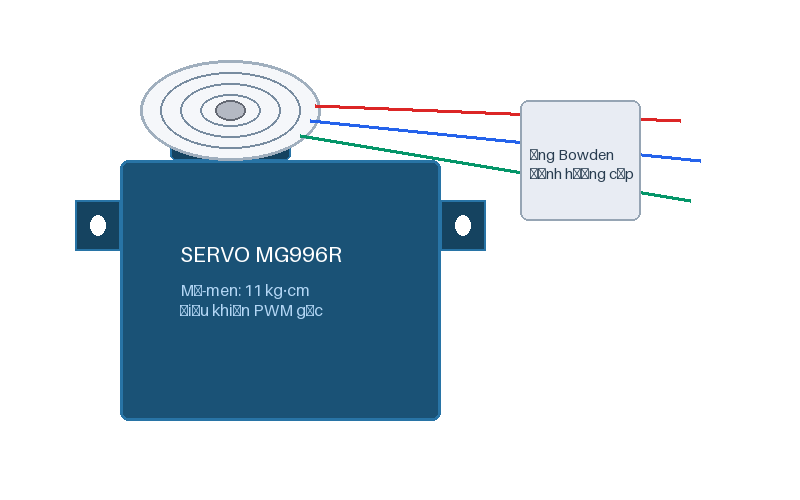
\includegraphics[width=4.1cm, height=2.6cm, keepaspectratio]{assets/servo_spool_assembly.png}\\[4pt]
  {\footnotesize 3 Động cơ Servo \& Tang cuốn cáp}
};

% 2. KHỐI THỊ GIÁC ĐÓN TRƯỚC (Căn giữa phía trên bộ điều khiển)
\node[stageCard, text width=7.2cm, minimum height=4.1cm] (vision) at (0, 4.4) {
  {\bfseries\normalsize\color{titleNavy} THỊ GIÁC ĐÓN TRƯỚC (DEPTH ANYTHING V2)}\\[4pt]
  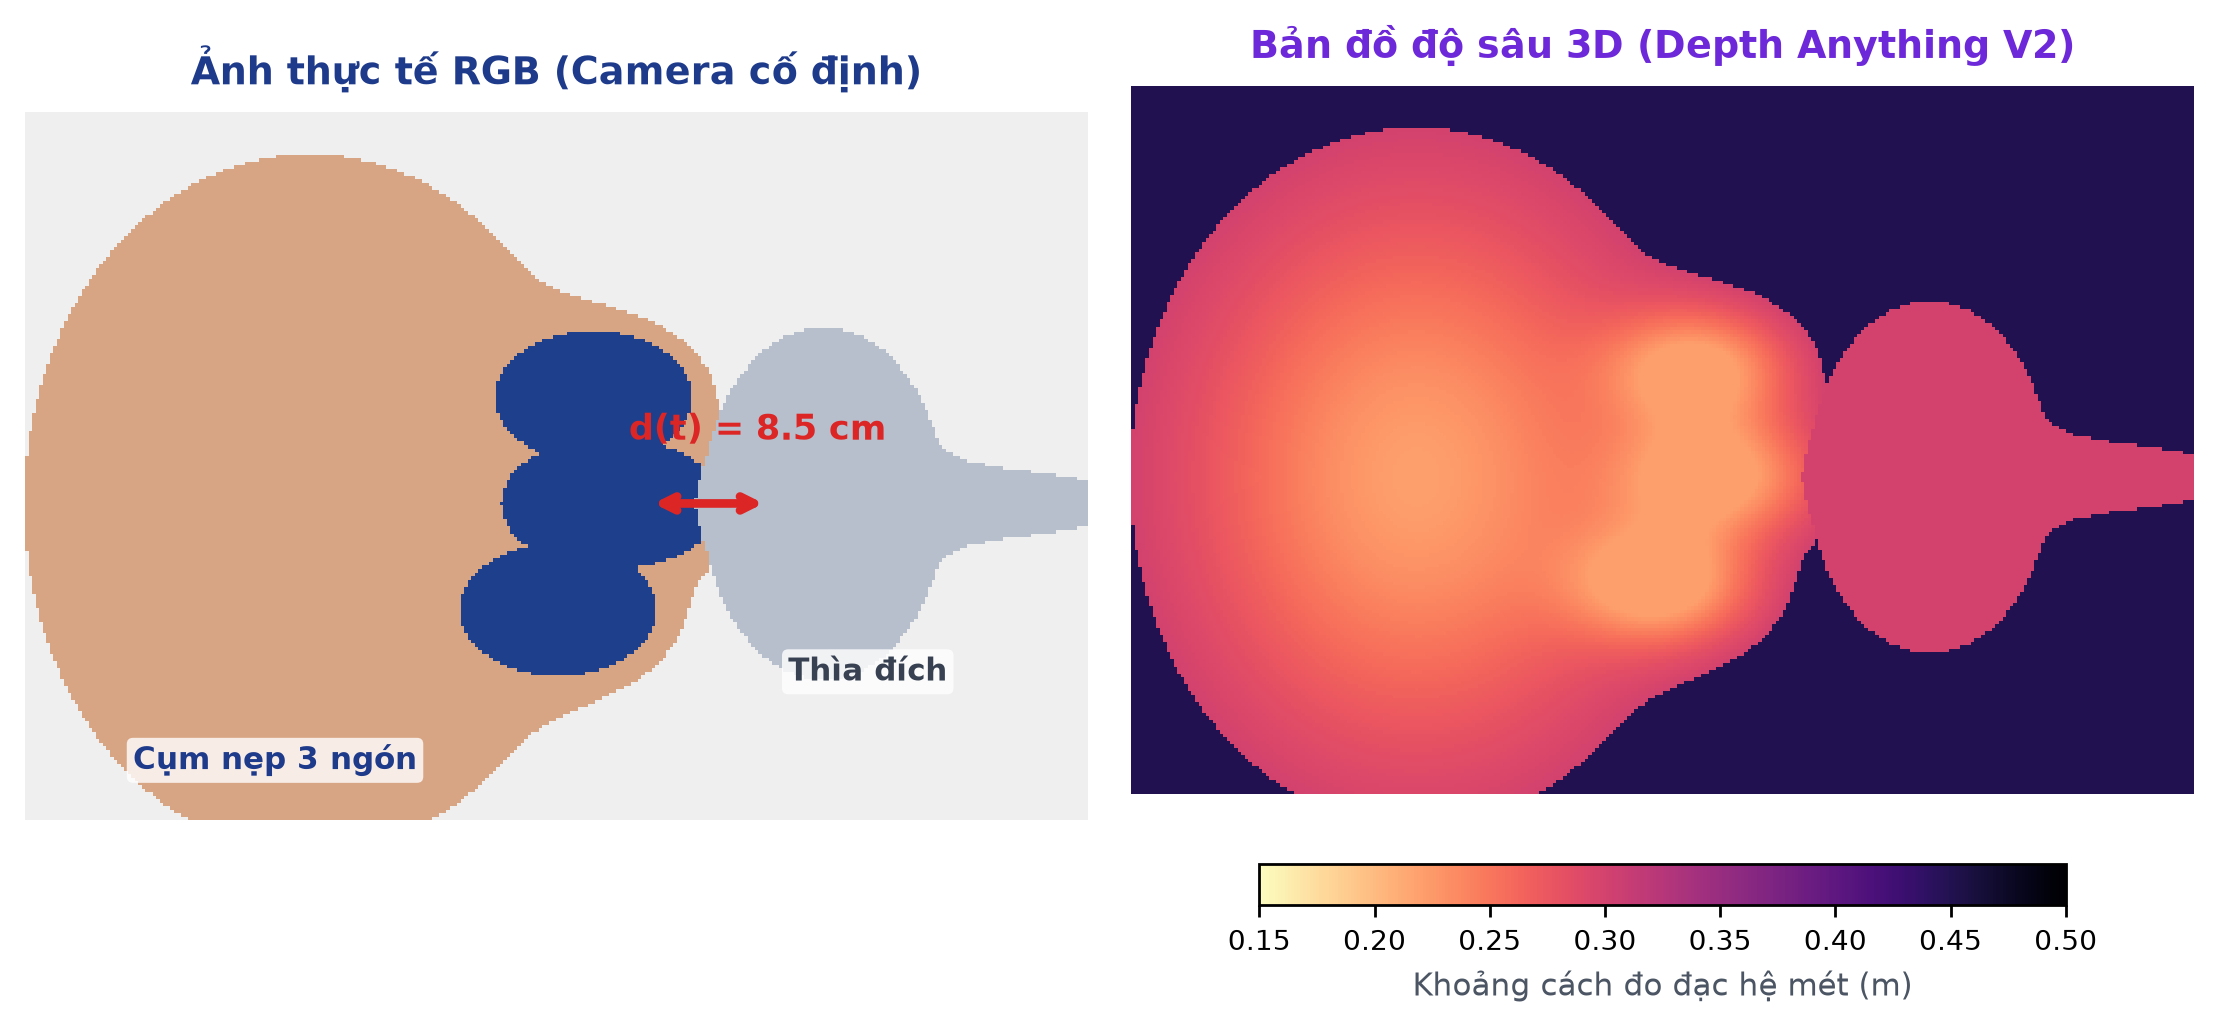
\includegraphics[width=6.8cm, height=2.7cm, keepaspectratio]{assets/depth_anything_scene.png}\\[4pt]
  {\footnotesize Camera RGB + Bản đồ độ sâu 3D (Đo cự ly tay -- vật \& Định thời TTC)}
};

% 3. CÁC MŨI TÊN LIÊN KẾT CHÍNH
\draw[arrowMain] (hand.east) -- node[tagLbl, above=2pt] {Lực \& Góc} (ctrl.west);
\draw[arrowMain] (ctrl.east) -- node[tagLbl, above=2pt] {Lệnh servo AAN} (act.west);
\draw[arrowMain] (vision.south) -- node[tagLbl, right=3pt] {Khẩu độ \& TTC đón trước} (ctrl.north);

% Camera quan sát từ nẹp tay lên khối thị giác
\draw[arrowDash] (hand.north) |- node[tagLbl, pos=0.75, above=2pt] {Camera quan sát cự ly 3D} (vision.west);

% 4. VÒNG PHẢN HỒI CƠ HỌC (Nằm phía dưới thanh thoát)
\draw[arrowDash] (act.south) -- ++(0, -0.85cm) coordinate (pAct) -- ($(pAct) - (11.2cm, 0)$) node[tagLbl, midway, below=3pt] {Vòng cơ học: Trợ lực kéo gập ngón / Nhả cáp duỗi ngón} -- (hand.south);

\end{tikzpicture}
\end{document}
